\documentclass{article}
\usepackage{graphicx,subcaption}
\usepackage[margin=2cm]{geometry}
\setlength{\parskip}{6pt}
\setlength{\parindent}{0pt}
\usepackage{tikz}
\usepackage{tikz-qtree}
\usetikzlibrary{positioning,arrows.meta,quotes,calc}
\tikzset{%
  arrow/.style    = { ->, >=Latex,  line width = 0.4mm, rounded corners, draw = black, every edge/.style={arrow} },
  arrow/.style    = { ->, >=Latex,  very thick, rounded corners,
                      fill = #1, draw = #1 },
  tbox/.style     = { fill = #1!20!white, draw = #1!80!white, thick, align = center,
                      minimum width = 0.8cm, minimum height = 0.6cm, node distance = 1.5cm },
  leaf/.style     = { fill = #1!20!white, draw = #1!80!white, thick, align = center, rounded corners = 0.3cm, grow = down,
                      minimum width = 1.2cm, minimum height = 0.6cm, node distance = 1.5cm }
}
\newcommand{\connectall}[2]{
  \foreach \s in {#1} {
    \foreach \t in {#2} {
      \draw[arrow,<->] (\s) -- (\t);
    }
  }
}
\graphicspath{{../../../outputs/figs/debug/propfrom/}}
% --------------------------------------------------------------------------------------------------
\title{Model Output: New Infections Ratio}
\author{Jesse Knight}
%%%%%%%%%%%%%%%%%%%%%%%%%%%%%%%%%%%%%%%%%%%%%%%%%%%%%%%%%%%%%%%%%%%%%%%%%%%%%%%%%%%%%%%%%%%%%%%%%%%%
\begin{document}
%%%%%%%%%%%%%%%%%%%%%%%%%%%%%%%%%%%%%%%%%%%%%%%%%%%%%%%%%%%%%%%%%%%%%%%%%%%%%%%%%%%%%%%%%%%%%%%%%%%%
\maketitle\vspace{-3em}
%%%%%%%%%%%%%%%%%%%%%%%%%%%%%%%%%%%%%%%%%%%%%%%%%%%%%%%%%%%%%%%%%%%%%%%%%%%%%%%%%%%%%%%%%%%%%%%%%%%%
\section{Objective}
In a heterogeneous system which includes turnover between sub-populations (groups),
the prevalence in any group is a function of both
``conduction'' (incidence) and ``convection'' (turnover).
Therefore we may be interested in the ratio of new infections among a given group
which arise from the force of infection versus from other groups via turnover.
%%%%%%%%%%%%%%%%%%%%%%%%%%%%%%%%%%%%%%%%%%%%%%%%%%%%%%%%%%%%%%%%%%%%%%%%%%%%%%%%%%%%%%%%%%%%%%%%%%%%
\section{System \& Proposed Output}
Consider the following open system, comprising sub-groups of $\mathcal{X}_i$ indexed by $i$,
internal flow rates $\zeta$, and force of infection $\lambda$:
\begin{figure}[h]
  \centering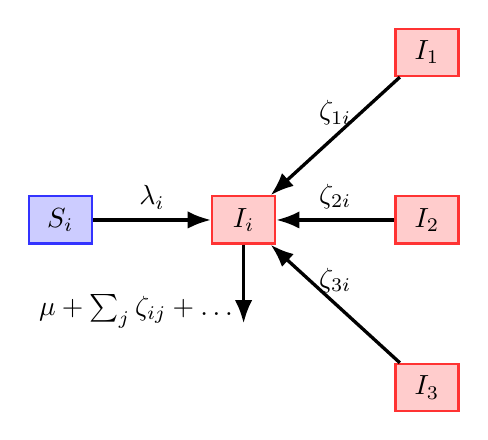
\begin{tikzpicture}
  \node(y)[tbox=red] {$I_i$};
  \node(s)[tbox=blue, left = of y]{$S_i$};
  \node(b)[tbox=red, right = of y]{$I_2$};
  \node(a)[tbox=red, above = of b]{$I_1$};
  \node(c)[tbox=red, below = of b]{$I_3$};
  \node(x)[below = of y]{};
  \draw[arrow,<-] (y) -- node[above] {$\lambda_{i}$} (s);
  \draw[arrow,<-] (y) -- node[above] {$\zeta_{1i}$} (a);
  \draw[arrow,<-] (y) -- node[above] {$\zeta_{2i}$} (b);
  \draw[arrow,<-] (y) -- node[above] {$\zeta_{3i}$} (c);
  \draw[arrow,->] (y) -- node[below left] {$\mu + \sum_j{\zeta_{ij}} + \dots$} (x);
\end{tikzpicture}
\end{figure}
\par
We define the new output as: the ratio of new infections in group $i$
which are due to turnover from group $j$
among all new infections in group $i$:
\begin{equation}
\mathcal{R}_{ji} = \frac{\zeta_{ji} {I}_j}{\lambda_i {S}_i + \sum_j \zeta_{ji} {I}_j}
\end{equation}
where $I$ indicates people living with HIV and $S$ indicates susceptible people.
%%%%%%%%%%%%%%%%%%%%%%%%%%%%%%%%%%%%%%%%%%%%%%%%%%%%%%%%%%%%%%%%%%%%%%%%%%%%%%%%%%%%%%%%%%%%%%%%%%%%
\section{Experiment}
We previously observed that turnover increases equilibrium prevalence among the low risk group.
In some cases, this also coincided with decreases in incidence among the same group --
an apparent contradiction for models without turnover.
However, here we can show that the increase in prevalence is attributable to
movement of infected people from high to low risk groups,
using the new output described above.
\par
Using the project model,
we computed the proportion of new infections among the low-activity group
which are attributable to turnover from \textit{any other group} (medium- and high-activity)
-- i.e. $\sum_j \mathcal{R}_{ij}$.
We varied the rate duration of infectiousness $\delta_I \in [5,10,20,50]$.
\par
Figure~\ref{fig:result} illustrates this result,
where we can see that up to 80\% individuals entering the ``infected \& low activity'' state
acquired their infections at a higher activity level.
For typical parameters $\delta_H \approx 10$ years and $\delta_I \approx 10$ years,
we see that about 20\% of infections in the low activity group were acquired elsewhere.
We also note that this proportion is proportional to the rate of treatment
(inverse of duration of infectiousness).
\par
As such, it is reasonable to conclude that increases in
prevalence among the low-activity group with turnover
(being on the order of 0 -- 50\%; \texttt{docs/debug/surface/surface.pdf})
can be mainly attributed to movement of infected individuals
from high-risk to low-risk groups.
\par
\begin{figure}
  \foreach \i in {05,10,20,50}{
    \begin{subfigure}{0.49\linewidth}
      \centering\includegraphics[width=\linewidth]{prop-I-in-L-from-HM-di=\i}
      \caption{Duration of infectiousness $\delta_I = \i$ years}
    \end{subfigure}
  }
  \caption{Proportion of new infections among the low-activity group from turnover}
  \label{fig:result}
\end{figure}
%%%%%%%%%%%%%%%%%%%%%%%%%%%%%%%%%%%%%%%%%%%%%%%%%%%%%%%%%%%%%%%%%%%%%%%%%%%%%%%%%%%%%%%%%%%%%%%%%%%%
\end{document}
%%%%%%%%%%%%%%%%%%%%%%%%%%%%%%%%%%%%%%%%%%%%%%%%%%%%%%%%%%%%%%%%%%%%%%%%%%%%%%%%%%%%%%%%%%%%%%%%%%%%